\documentclass[journal,12pt,twocolumn]{IEEEtran}
\usepackage{amsmath,amssymb,amsfonts,amsthm}
\usepackage{txfonts}
\usepackage{tkz-euclide}
\usepackage{listings}
\usepackage{gvv}
\usepackage[latin1]{inputenc}
\usepackage{adjustbox}
\usepackage{array}
\usepackage{tabularx}
\usepackage{pgf}
\usepackage{lmodern}
\usepackage{circuitikz}
\usepackage{tikz}
\usepackage{graphicx}

\begin{document}
\bibliographystyle{IEEEtran}

\vspace{3cm}

\title{}
\author{EE23BTECH11054 -  Sai Krishna Shanigarapu$^{*}$
}
\maketitle
\newpage
\bigskip

% \renewcommand{\thefigure}{\theenumi}
% \renewcommand{\thetable}{\theenumi}

\section*{Gate EE 2023}
54. \hspace{2pt}The circuit shown in the figure is initially in the steady state with the switch K in open condition and $\overline{K}$ in closed condition. The switch K is closed and $\overline{K}$ is opened simultaneously at the instant $t = t_1$, where $t_1 > 0$. The minimum value of $t_1$ in milliseconds such that there is no transient in the voltage across the 100 $\mu F$ capacitor, is \rule{1cm}{0.15mm} (Round off to 2 decimal places).\\ (GATE EE 2023)

\begin{figure}[h!]
  \centering
  \resizebox{0.8\columnwidth}{!}{\begin{circuitikz}[american]
       \draw (0,0) to [R=10$\Omega$] (0,5) to [short] (4,5);
       \draw (0,0) to [short] (4,0) to [isource, l=\large{{$\sin\brak{1000t}$}}] (4,5) to [short] (7,5) to [cspst=K] ++(0,-3);
       \draw (7,2) to [short] (7,0) to [short] (4,0);
       \draw (7,5) to [short] (11,5) to [curved capacitor=100$\mu$F] (11,0);
       \draw (7,0) to [ospst=$\overline{K}$] ++(4,0);
       \draw (7,0) to [short] (8,1.5) to [R=10$\Omega$] (9.3,1.5) to [battery2 = 5V] (10,1.5) to [short] (11,0);
\end{circuitikz}

}
\end{figure}

\solution

Case(i) Switch K is open and $\overline{K}$ is closed.
\begin{figure}[h!]
  \centering
  \resizebox{0.50\columnwidth}{!}{    \begin{circuitikz}[american]
        \draw (0,7) to [R=10$\Omega$] (0,2) to [short] (3,2) to [isource, l=$1\angle{0^\circ}$] (3,7) to [short] (0,7);
        \draw (3,7) to [short, i=$I_1$] (7,7);
        \draw (3,2) to [short] (7,2);
        \draw (7,7) -- ++(0,-1.5)
        to [open, v=$V_1$, o-o] ++(0,-1.5) -- ++(0,-2);
\end{circuitikz}

}
\end{figure}

Using Current divider rule,
\begin{align}
    i_c\brak{s} &= \brak{\frac{10^3}{s^2 + 10^6}}\brak{\frac{10}{10 + \frac{10^4}{s}}}\\
    &= \frac{10^3 s}{\brak{s^2 + 10^6}\brak{s + 10^3}}\\
    V_1\brak{s} &= \frac{10^7}{\brak{s^2 + 10^6} \brak{s + 10^3}} 
\end{align}



\newpage
Case(ii) Switch K is closed and $\overline{K}$ is open.

\begin{figure}[h!]
  \centering
  \resizebox{0.55\columnwidth}{!}{%\begin{circuitikz}[american]
        %\draw (0,0) to [R=10$\Omega$] (1.5,0) to [battery2=5V] (4,0);
        %\draw (0,0) to [short] (0,3) to [short] (4,3) to [C=100$\mu$F, %v=$V_c\brak{\infty}$] (4,0) ;
%\end{circuitikz}

\begin{circuitikz}[american]
    \draw (0,0) to [R=10$\Omega$] (1.5,0) to [battery2=$\frac{5}{s}$] (4,0);
    \draw[<-, thick] (1.5,1) arc (-90:90:0.5) node[midway, left] {$I(s)$};
    \draw (0,0) to [short] (0,3) to [short] (4,3) to [C=$\frac{10^4}{s}$, v=$V_c\brak{s}$] (4,0);
\end{circuitikz}

}
\end{figure}



\begin{align}
    I\brak{s} &= \frac{\frac{5}{s} - V_1\brak{s}}{10 + \frac{10^4}{s}}\\
    V_c\brak{s} &= \frac{5}{s} - 10\brak{\frac{5-V_1\brak{s}}{1+10^{-3}s}}
\end{align}

For transient analysis,
\begin{align}
    \frac{5-V_1\brak{s}}{1+10^{-3}s} &= 0\\
    \implies V_1\brak{s} &= 5\\
    \frac{10^7}{\brak{s^2+10^6}\brak{s+10^3}} &= \frac{5}{s}\\
    \frac{5}{s+10^3} + \frac{10^3-s}{s^2 + 10^6} &= \frac{5}{s}\\
    \frac{-s}{s^2+10^6} + \frac{10^3}{s^2 + 10^6} + \frac{1}{s+10^3} &= \frac{1}{s}\\
    -\cos\brak{1000t_1}+\sin\brak{1000t_1}+e^{-10^3 t_1} &= 1\\
    \implies t_1 \approx 1.57\text{msec}
\end{align}



\begin{table}[ht]
    \setlength{\arrayrulewidth}{0.3mm}
\setlength{\tabcolsep}{15pt}
\renewcommand{\arraystretch}{1.4}

\resizebox{10cm}{!}{
\begin{tabular}{|c|c|c|}
\hline

Symbol & description & value\\
\hline
$V_C\brak{\infty}$ & Voltage across capacitor after long time & $5V$\\
\hline
$\tau$ & Time constant & 1 msec\\
\hline
%$V_c\brak{t}$ & Voltage across capacitor at time t & $5 + \brak{7.07\sin \brak{100t - 45^\circ}-5}e^{-\brak{t-t_1}/ \tau}$\\
%\hline
R & Resistance & 10$\Omega$\\
\hline
C & capacitance & 100$\mu$F\\
\hline
f & frequency of the current source & $\frac{500}{\pi}$\\
\hline


\end{tabular}
}

    \vspace{0.5cm}
    \caption{Laplace transforms}
    \label{tab:Gate.ee.54.1}
\end{table}

\begin{figure}[ht]
    \centering
    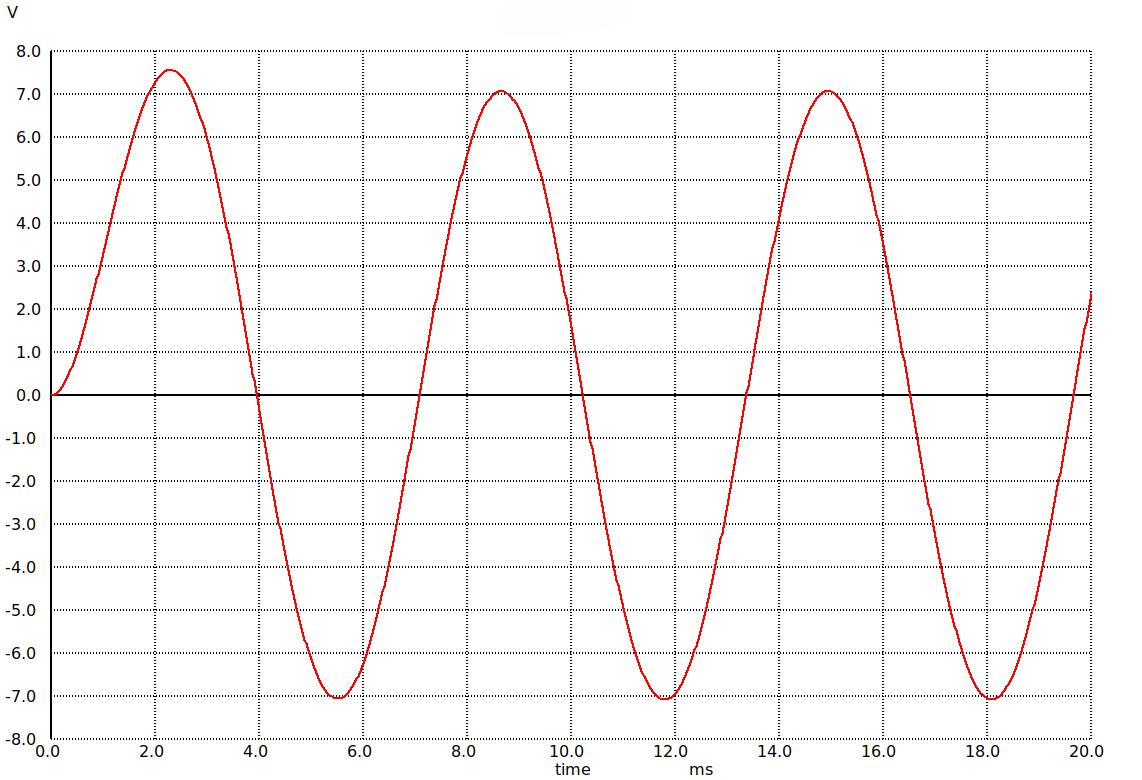
\includegraphics[width=1\columnwidth]{figs/fig1.png}
    \caption{plot of $V_1$ in case(i)}
    \label{fig:fig1.gate.ee.23.54}
\end{figure}

\begin{figure}[ht]
    \centering
    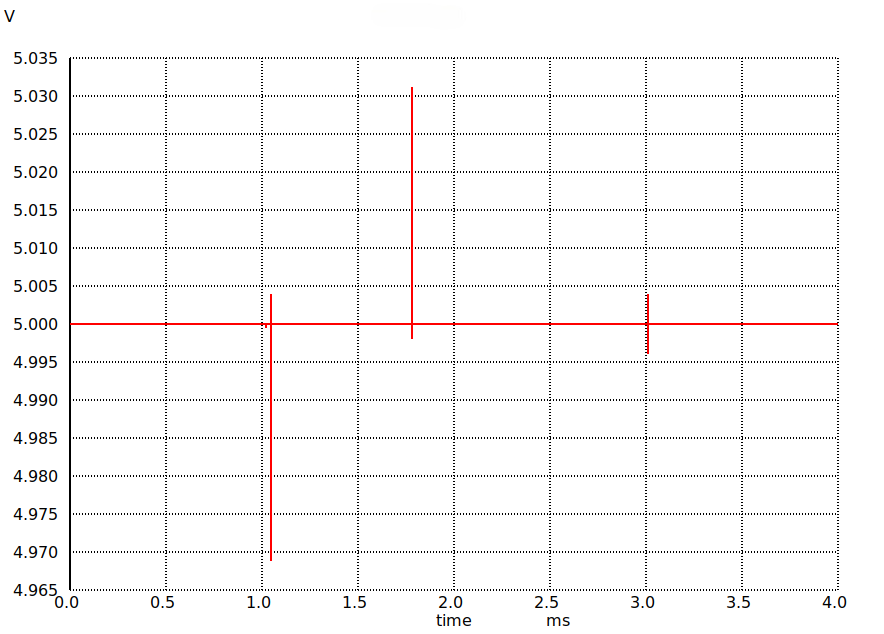
\includegraphics[width=1\columnwidth]{figs/fig2.png}
    \caption{plot of $V_c$ in case(ii)}
    \label{fig:fig2.gate.ee.23.54}
\end{figure}

\end{document}
